\documentclass[aspectratio=169]{beamer}
\usetheme{Madrid}
\usepackage{calc}
\usecolortheme{whale}
\usepackage{tikz}
\usetikzlibrary{positioning}
\usepackage{hyperref}
\usepackage{graphicx}
\usepackage{colortbl}

\title{Welcome to Ethics: An Introduction}
\author{Brendan Shea, PhD}
\institute{Rochester Community and Technical College}
\date{Spring 2025}

\begin{document}

\begin{frame}
\titlepage
\end{frame}

\begin{frame}{Welcome to Ethics: An Introduction}
\begin{itemize}
\item \textbf{Ethics} is central to many of the most pressing challenges facing our society today, from artificial intelligence governance to climate change response.
\item Throughout this course, we will explore both \emph{timeless questions} about the nature of right and wrong and their application to \emph{contemporary issues}.
\item Our journey begins with Plato, whose insights about knowledge, reality, and justice remain remarkably relevant to modern debates about social media, virtual reality, and political polarization.
\item We will develop tools for careful ethical reasoning that you can apply in your personal life, professional career, and role as a citizen.
\end{itemize}
\end{frame}

\begin{frame}{From Plato's Republic}
\begin{quote}
\small
"Until philosophers are kings, or the kings and princes of this world have the spirit and power of philosophy, and political greatness and wisdom meet in one, and those commoner natures who pursue either to the exclusion of the other are compelled to stand aside, cities will never have rest from their evils—no, nor the human race, as I believe—and then only will this our State have a possibility of life and behold the light of day."
\end{quote}
\vspace{0.5cm}
\begin{itemize}
\item This famous passage captures Plato's vision that \textbf{genuine knowledge} must guide political power.
\item It raises timeless questions about the relationship between \emph{expertise}, \emph{ethics}, and \emph{governance}.
\item These themes resonate with modern debates about the role of scientific expertise in policy-making.
\end{itemize}
\end{frame}

\begin{frame}{What Is Ethics? Normative vs. Descriptive}
\begin{itemize}
\item \textbf{Descriptive ethics} examines how people actually behave and what they believe about right and wrong—for instance, studying how moral attitudes toward same-sex marriage have evolved over time.
\item \textbf{Normative ethics} asks what we \emph{should} do and how we \emph{ought} to live—like debating whether we have an ethical obligation to reduce our carbon footprint.
\item While scientific research can tell us about the \emph{consequences} of our actions (descriptive), it cannot by itself tell us what we \emph{ought} to do (normative).
\item Understanding this distinction helps us avoid the naturalistic fallacy—the mistake of inferring what \emph{ought} to be solely from what \emph{is}.
\end{itemize}
\end{frame}

\begin{frame}{Theoretical vs. Applied Ethics}
\begin{itemize}
\item \textbf{Theoretical ethics} explores fundamental questions about the nature of morality—for example, whether moral truths are objective or whether they depend on cultural context.
\item \textbf{Applied ethics} takes these theoretical insights and uses them to address specific real-world problems, like the ethical implications of autonomous weapons or genetic engineering.
\item The relationship between theory and practice is \emph{bidirectional}—our theoretical understanding informs how we approach practical problems, while practical challenges often reveal the limitations of our theories.
\item Consider how debates about AI alignment combine deep theoretical questions about the nature of intelligence and consciousness with urgent practical concerns about safety and governance.
\item The most effective ethical reasoning often moves back and forth between theoretical principles and specific cases, refining both in light of the other.
\end{itemize}
\end{frame}

\begin{frame}{The Structure of Ethical Inquiry}
\begin{center}
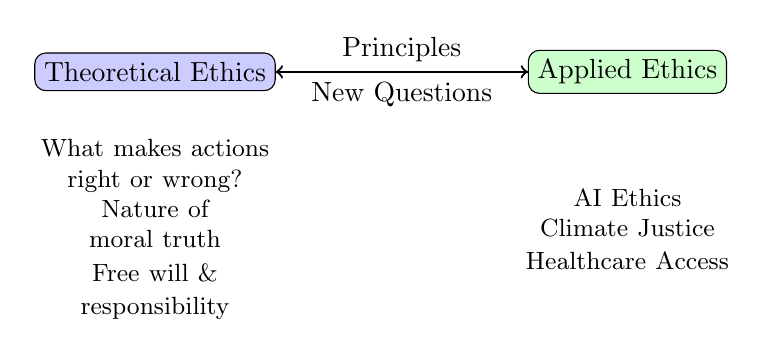
\begin{tikzpicture}
    % Create main nodes
    \node[draw, rectangle, rounded corners, fill=blue!20] (theoretical) {Theoretical Ethics};
    \node[draw, rectangle, rounded corners, fill=green!20] (applied) at (6,0) {Applied Ethics};
    
    % Examples underneath
    \node[text width=3cm, align=center] (theory_ex) at (0,-2)
        {\small What makes actions right or wrong?\\ Nature of moral truth\\ Free will \& responsibility};
    \node[text width=3cm, align=center] (applied_ex) at (6,-2)
        {\small AI Ethics\\ Climate Justice\\ Healthcare Access};
    
    % Bidirectional arrows
    \draw[->, thick] (theoretical) -- node[above] {Principles} (applied);
    \draw[->, thick] (applied) -- node[below] {New Questions} (theoretical);
\end{tikzpicture}
\end{center}
\end{frame}

\begin{frame}{Why Study Plato in Ethics?}
\begin{itemize}
\item Plato's dialogues present ethical questions in a uniquely accessible yet profound way, using analogies and stories that still resonate with modern readers.
\item His critique of \textbf{moral relativism} remains relevant to contemporary debates about cultural differences and universal human rights.
\item Plato's insights about education and moral development have been supported by modern \textbf{psychological research} on moral reasoning and character formation.
\item His analysis of how social structures shape individual behavior anticipates modern discussions about \emph{systemic injustice} and institutional reform.
\item The \textbf{dialectical method} he employs—carefully examining arguments through dialogue—provides a model for thoughtful ethical discourse in our polarized times.
\end{itemize}
\end{frame}

\begin{frame}{Plato: A Brief Historical Context}
\begin{itemize}
\item Plato (c. 428-348 BCE) lived during a period of significant political upheaval in Athens, including the aftermath of the Peloponnesian War and the execution of his mentor \textbf{Socrates}.
\item His philosophical work was shaped by the \emph{crisis of democracy} he witnessed, leading him to question how societies can maintain justice and stability while avoiding both tyranny and mob rule.
\item The intellectual environment of 5th century BCE Athens included competing schools of thought like the \textbf{Sophists}, who taught that morality was merely a matter of convention and power.
\item Plato founded the \emph{Academy}—often considered the first Western university—establishing a tradition of systematic philosophical education that continues today.
\end{itemize}
\end{frame}

\begin{frame}{Key Concepts in Plato's Philosophy}
\begin{itemize}
\item At the heart of Plato's \textbf{moral realism} is the idea that moral truth is \textbf{objective and knowable} through rational inquiry—similar to how we can discover mathematical truths.
\item His theory of \emph{Forms} suggests that concepts like justice, beauty, and goodness have a reality independent of our opinions about them—challenging both moral relativism and subjectivism.
\item Plato argues that \emph{ethical knowledge requires careful education} of both reason and character, anticipating modern research on the role of emotion in moral decision-making.
\item The \emph{Socratic method} of questioning assumptions and examining arguments remains a powerful tool for ethical inquiry, especially in our era of social media echo chambers.
\item Understanding virtue requires studying both \emph{individual psychology} and social structures—a holistic approach relevant to modern debates about personal versus institutional responsibility.
\end{itemize}
\end{frame}

\begin{frame}
    \frametitle{The Cave}
    \begin{quotation}
    "And now, I said, let me show in a figure how far our nature is enlightened or unenlightened:—Behold! human beings living in a underground den, which has a mouth open towards the light and reaching all along the den; here they have been from their childhood, and have their legs and necks chained so that they cannot move, and can only see before them, being prevented by the chains from turning round their heads. Above and behind them a fire is blazing at a distance, and between the fire and the prisoners there is a raised way; and you will see, if you look, a low wall built along the way, like the screen which marionette players have in front of them, over which they show the puppets.
    
    \end{quotation}
    \vspace{0.5cm}
    \small{-- Republic, Book 7}
\end{frame}

\begin{frame}
    \frametitle{The Cave, II}
    \begin{quotation}
    "This entire allegory, I said, you may now append, dear Glaucon, to the previous argument; the prison-house is the world of sight, the light of the fire is the sun, and you will not misapprehend me if you interpret the journey upwards to be the ascent of the soul into the intellectual world according to my poor belief, which, at your desire, I have expressed—whether rightly or wrongly God knows."
    ... 
    "Whether true or false, my opinion is that in the world of knowledge the idea of good appears last of all, and is seen only with an effort; and, when seen, is also inferred to be the universal author of all things beautiful and right, parent of light and of the lord of light in this visible world, and the immediate source of reason and truth in the intellectual; and that this is the power upon which he who would act rationally either in public or private life must have his eye fixed."
    \end{quotation}
    \vspace{0.5cm}
    \small{-- Republic, Book 7}
\end{frame}



\begin{frame}{The Cave Analogy: What Is It?}
\begin{itemize}
\item The \textbf{Allegory of the Cave} appears in Book VII of Plato's Republic, presenting a powerful metaphor that explores the relationship between appearance and reality.
\item Prisoners are chained in a cave since childhood, only able to see \emph{shadows} projected on the wall by artificial objects—representing how our understanding is often limited by our circumstances and education.
\item One prisoner breaks free and makes a difficult journey toward the sun, experiencing stages of increasing illumination—paralleling the challenges of philosophical education.
\item The freed prisoner's return to help others illustrates both the \emph{social responsibility} of the philosopher and the challenges of sharing difficult truths.
\item This metaphor remains powerful today, helping us think about filter bubbles, echo chambers, and the challenge of seeing beyond our own limited perspectives.
\end{itemize}
\end{frame}

\begin{frame}{The Cave Analogy: Modern Applications}
\begin{itemize}
\item Contemporary digital environments often function like Plato's cave—creating compelling but potentially misleading representations of reality.
\item Social media algorithms create personalized \emph{echo chambers} that can limit our exposure to diverse viewpoints and reinforce existing beliefs.
\item The rise of sophisticated AI-generated content raises new questions about the relationship between appearance and reality—making Plato's concerns about illusion more relevant than ever.
\item Like Plato's prisoners, we may become \emph{comfortable} with our limited perspective, resisting information that challenges our existing worldview.
\item The cave analogy helps us think critically about how technology shapes our understanding of truth, justice, and reality in the digital age.
\end{itemize}
\end{frame}

\begin{frame}{The Cave's Stages of Understanding}
\begin{itemize}
\item Plato presents a \textbf{hierarchical model} of knowledge and understanding, with distinct stages representing different levels of ethical insight.
\item Each stage requires both \emph{intellectual growth} and \emph{character development}—we must become different kinds of people to access deeper ethical truths.
\item The journey is both personal and social—individual enlightenment should lead to efforts to improve the broader community.
\item Modern psychology confirms Plato's insight that changing deeply held beliefs requires both rational understanding and emotional development.
\end{itemize}
\end{frame}

\begin{frame}{Stages of Knowledge in Plato's Cave}
\begin{center}
\begin{tabular}{|p{2.5cm}|p{4cm}|p{4cm}|}
\hline
\textbf{Stage} & \textbf{Cave Metaphor} & \textbf{Modern Example} \\
\hline
\emph{Illusion} & Shadows on cave wall & Social media echo chambers, clickbait headlines \\
\hline
\emph{Common Opinion} & Artificial objects casting shadows & Conventional wisdom, popular beliefs \\
\hline
\emph{Scientific Understanding} & Stars and moon outside cave & Empirical research, data analysis \\
\hline
\emph{Philosophical Wisdom} & The sun (Form of the Good) & Comprehensive ethical understanding \\
\hline
\end{tabular}
\end{center}
\vspace{0.3cm}
\begin{itemize}
\item Each stage represents both increased \textbf{knowledge} and greater \emph{responsibility} to help others achieve understanding
\item Movement between stages requires both intellectual and moral development
\end{itemize}
\end{frame}
\begin{frame}{Moral Psychology: The Tripartite Soul}
\begin{itemize}
\item Plato's psychological theory divides the soul into \textbf{three distinct parts}, each with its own desires and motivations.
\item \textbf{Reason} (logistikon) seeks truth and knowledge—like the scientist pursuing understanding or the philosopher seeking wisdom.
\item \textbf{Spirit} (thymoeides) pursues honor and recognition—manifesting in our sense of justice, competitive drive, and moral indignation.
\item The \textbf{appetitive part} (epithymetikon) seeks pleasure and satisfaction of basic desires—from food and drink to material wealth.
\item Modern psychology confirms this complex view of human motivation, recognizing both rational and non-rational influences on moral behavior.
\end{itemize}
\end{frame}

\begin{frame}{Harmony and Conflict in the Soul}
\begin{itemize}
\item For Plato, \textbf{moral virtue} requires proper ordering of the soul's parts—reason should guide, supported by spirit, with appetites properly constrained.
\item Internal conflict occurs when different parts pull us in opposing directions—like when we know we should study (reason) but want to watch TV (appetite).
\item The \emph{spirited element} plays a crucial role in moral development by naturally allying with reason against excessive appetites—similar to how our sense of pride can help us resist temptation.
\item This model helps explain common patterns of \textbf{moral failure}, such as when knowledge of what's right fails to motivate action because our emotions and desires aren't properly aligned.
\item Modern approaches to character education often echo Plato's insight that moral development requires training both intellectual and emotional capacities.
\end{itemize}
\end{frame}

\begin{frame}{Plato's Ethical Realism: The Forms}
\begin{itemize}
\item Plato argues that moral concepts like justice and goodness have \textbf{objective reality} independent of human opinions or cultural conventions.
\item The Forms are perfect, unchanging patterns that particular things imperfectly exemplify—just as all circles we draw are imperfect copies of the ideal circle.
\item This view challenges both moral relativism ("\emph{justice is just what each society decides}") and \textbf{moral skepticism} ("there are no moral truths").
\item Understanding the Forms requires both intellectual training and character development—similar to how appreciating great art or music requires both knowledge and refined sensibility.
\item While Plato's metaphysics may seem abstract, his core insight that moral truth is objective and discoverable remains influential in contemporary ethics.
\end{itemize}
\end{frame}
\begin{frame}{The Structure of the Soul}
\begin{center}
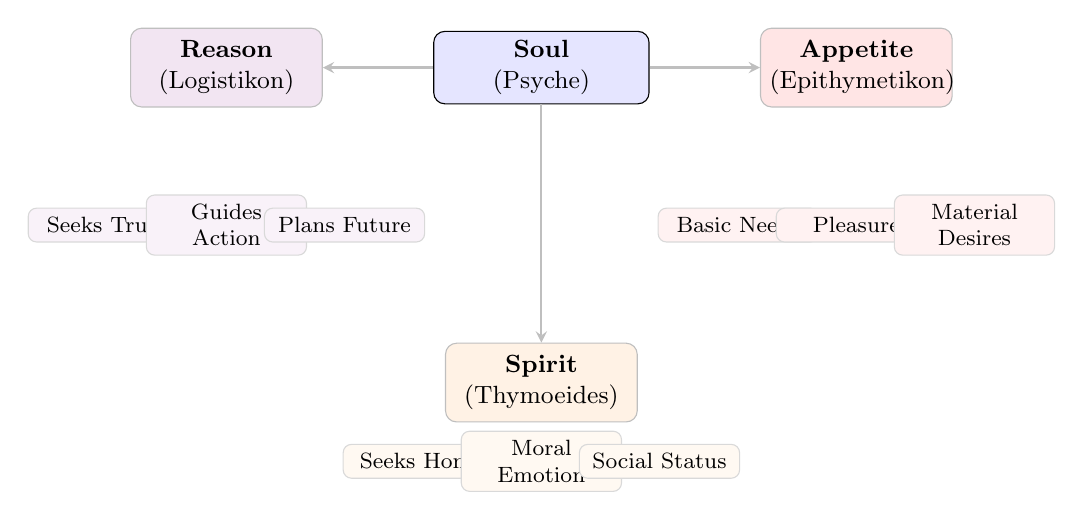
\begin{tikzpicture}[
    % Modern styling
    node distance=2cm,
    every node/.style={
        text width=2.5cm,
        align=center,
        font=\small
    },
    % Custom styles for different levels
    level 1/.style={
        rounded corners,
        draw=gray!50,
        fill=white,
        minimum height=1cm,
        text width=2.2cm
    },
    level 2/.style={
        rounded corners=3pt,
        draw=gray!30,
        fill=white,
        text width=1.8cm,
        font=\footnotesize
    }
]
    % Central node
    \node[draw, fill=blue!10, rounded corners] (soul) {\textbf{Soul}\\(Psyche)};
    
    % Main parts of the soul
    \node[level 1, fill=violet!10] (reason) at (-4,0) {\textbf{Reason}\\(Logistikon)};
    \node[level 1, fill=orange!10] (spirit) at (0,-4) {\textbf{Spirit}\\(Thymoeides)};
    \node[level 1, fill=red!10] (appetite) at (4,0) {\textbf{Appetite}\\(Epithymetikon)};
    
    % Connect main parts
    \draw[-stealth, thick, gray!50] (soul) -- (reason);
    \draw[-stealth, thick, gray!50] (soul) -- (spirit);
    \draw[-stealth, thick, gray!50] (soul) -- (appetite);
    
    % Reason's attributes
    \node[level 2, fill=violet!5] at (-5.5,-2) {Seeks Truth};
    \node[level 2, fill=violet!5] at (-4,-2) {Guides Action};
    \node[level 2, fill=violet!5] at (-2.5,-2) {Plans Future};
    
    % Spirit's attributes
    \node[level 2, fill=orange!5] at (-1.5,-5) {Seeks Honor};
    \node[level 2, fill=orange!5] at (0,-5) {Moral Emotion};
    \node[level 2, fill=orange!5] at (1.5,-5) {Social Status};
    
    % Appetite's attributes
    \node[level 2, fill=red!5] at (2.5,-2) {Basic Needs};
    \node[level 2, fill=red!5] at (4,-2) {Pleasure};
    \node[level 2, fill=red!5] at (5.5,-2) {Material Desires};
\end{tikzpicture}
\end{center}
\end{frame}

\begin{frame}{The Form of the Good}
\begin{itemize}
\item The Form of the Good stands at the pinnacle of Plato's metaphysical system, playing a role analogous to the \textbf{sun in the Cave allegory}.
\item Just as the sun makes vision possible and gives life to living things, the Good makes \emph{knowledge possible} and gives reality to the other Forms.
\item Understanding the Good requires extensive preparation—including mathematics, dialectic, and practical experience—making it accessible only after years of \textbf{rigorous study}.
\item Modern parallels might include the search for \emph{fundamental ethical principles} that could guide decision-making across different contexts.
\item While complete knowledge of the Good may be difficult to achieve, Plato argues that even partial understanding can improve our ethical reasoning.
\end{itemize}
\end{frame}

\begin{frame}
    \frametitle{Justice and the Individual}
    \begin{quotation}
    ``Consider further - most foolish Socrates - that the just is always a loser in comparison with the unjust. First of all, in private contracts: wherever the unjust is the partner of the just you will find that, when the partnership is dissolved, the unjust entity always has more and the just less [...] when there is an income tax, the just man will pay more and the cunning unjust usually less on the same amount of income.''
    \end{quotation}
    \vspace{0.5cm}
    \small{-- Book I, 351d}
\end{frame}

\begin{frame}{Plato vs. Ethical Egoism}
\begin{itemize}
\item \textbf{Ethical egoism}—the view that we should act purely in our own self-interest—was defended by some of Plato's contemporaries, particularly Thrasymachus in Book I of the Republic.
\item Plato argues that this view rests on a \emph{fundamental misunderstanding} of human nature and happiness—we are inherently social beings whose well-being depends on living in a just community.
\item The tripartite soul theory suggests that purely self-interested behavior represents a \textbf{dysfunction} where appetite dominates reason and spirit.
\item Plato explores this using the myth of the \textbf{Ring of Gyges}, which suggests that many people will act unjustly if they can do so without facing consequences.
\item Plato's response to ethical egoism anticipates modern research showing that prosocial behavior often promotes individual well-being.
\end{itemize}
\end{frame}

\begin{frame}{Plato vs. Cultural Relativism}
\begin{itemize}
\item Cultural relativism—the view that moral truth is relative to particular societies—was articulated by the \textbf{Sophists} in Plato's time.
\item Plato argues that this view is both \emph{self-contradictory} (is relativism itself only relatively true?) and dangerous for practical ethics.
\item The Cave allegory suggests that cultural conventions may be like shadows on the wall—reflecting but \textbf{distorting} underlying moral reality.
\item This remains relevant to contemporary debates about \emph{universal human rights} versus cultural traditions.
\item Plato's position suggests we can acknowledge cultural differences while still seeking common ethical principles—similar to modern human rights frameworks.
\end{itemize}
\end{frame}

\begin{frame}{Plato vs Divine Command Theory}
    \begin{itemize}
    \item Divine Command Theory—the view that morality is simply whatever the gods command—is challenged by Plato in the \textbf{Euthyphro} dialogue through the famous dilemma.
    \item Plato argues that this view faces a crucial question: Is something moral \emph{because} the gods command it, or do the gods command it \textbf{because} it is moral?
    \item If morality is based purely on divine command, it becomes arbitrary; if gods choose what to command based on independent moral truths, then morality must exist separately from divine will.
    \item This critique remains relevant to modern debates about the relationship between \emph{religion and ethics}, particularly in pluralistic societies.
    \item Plato's analysis suggests that even religious ethics must engage with rational moral reasoning—anticipating modern philosophical theology.
    \end{itemize}
    \end{frame}
    
    \begin{frame}{Plato vs Majoritarianism}
    \begin{itemize}
    \item Majoritarianism—the view that whatever the majority decides is right—is critiqued by Plato through his analysis of \textbf{democracy} in the Republic.
    \item Plato argues that moral truth cannot be determined by popular vote any more than scientific or mathematical truth—expertise and \emph{rational investigation} are necessary.
    \item The Ship of State allegory suggests that letting the majority rule without wisdom is like letting passengers control a ship instead of a trained \textbf{navigator}.
    \item This remains relevant to contemporary debates about the limits of \emph{democratic decision-making}, particularly regarding technical or ethical issues.
    \item Plato's critiques of democracy anticipate modern concerns about the \textbf{limits of popular will} in complex ethical and technical matters.
    \end{itemize}
    \end{frame}

\begin{frame}{Justice in the Individual and the State}
\begin{itemize}
\item Plato draws a crucial parallel between the structure of the \textbf{just soul} and the \textbf{just state}, arguing that both require proper ordering of their parts.
\item Just as reason should guide the individual soul, the \textbf{philosopher-rulers} (representing wisdom) should guide the state.
\item The \textbf{guardian class} corresponds to spirit in the soul, while the productive class corresponds to appetite—each playing essential but distinct roles.
\item This model raises enduring questions about the relationship between \emph{individual virtue} and \emph{social justice}.
\item Modern applications include debates about technocracy versus democracy, and the role of expertise in public policy.
\end{itemize}


\end{frame}

\begin{frame}{Modern Parallels to Plato's Cave}
\begin{center}
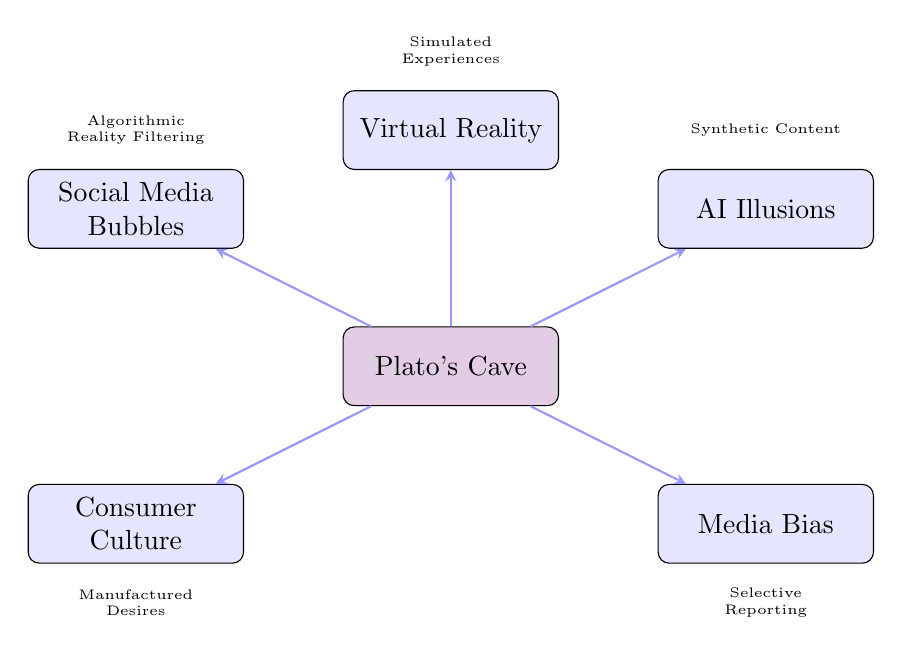
\begin{tikzpicture}[
    box/.style={
        draw,
        rounded corners,
        fill=blue!10,
        text width=2.5cm,
        align=center,
        minimum height=1cm
    },
    arrow/.style={
        ->,
        thick,
        >=stealth,
        blue!40
    }
]
    % Core concept
    \node[box, fill=violet!20] (cave) at (0,0) {Plato's Cave};
    
    % Modern parallels (in a circle around the center)
    \node[box] (social) at (-4,2) {Social Media Bubbles};
    \node[box] (vr) at (0,3) {Virtual Reality};
    \node[box] (ai) at (4,2) {AI Illusions};
    \node[box] (media) at (4,-2) {Media Bias};
    \node[box] (consumerism) at (-4,-2) {Consumer Culture};
    
    % Connecting arrows
    \draw[arrow] (cave) -- (social);
    \draw[arrow] (cave) -- (vr);
    \draw[arrow] (cave) -- (ai);
    \draw[arrow] (cave) -- (media);
    \draw[arrow] (cave) -- (consumerism);
    
    % Adding small explanatory notes
    \node[font=\tiny, text width=2cm, align=center] at (-4,3) {Algorithmic Reality Filtering};
    \node[font=\tiny, text width=2cm, align=center] at (0,4) {Simulated Experiences};
    \node[font=\tiny, text width=2cm, align=center] at (4,3) {Synthetic Content};
    \node[font=\tiny, text width=2cm, align=center] at (4,-3) {Selective Reporting};
    \node[font=\tiny, text width=2cm, align=center] at (-4,-3) {Manufactured Desires};
\end{tikzpicture}
\end{center}
\end{frame}

\begin{frame}{Modern Caves: The Matrix}
    \begin{itemize}
        \item In "The Matrix," humans live in a simulated reality while machines harvest their bodies for energy; protagonist Neo discovers this truth and joins a resistance movement.
        \item The character Cypher, who chooses illusion over reality, represents the \emph{psychological challenge} of confronting uncomfortable truths.
        \item Like Plato's freed prisoner, Neo faces both the personal struggle of accepting reality and the social responsibility of helping others.
        \item The film explores Platonic themes about the relationship between \emph{physical} and \emph{digital} reality that have become increasingly relevant.
        \item The choice between comfortable illusion and difficult truth remains as challenging today as in Plato's time.
        \end{itemize}
    \end{frame}

    \begin{frame}{Modern Caves:The Truman Show}
        \begin{itemize}
        \item Truman Burbank lives in a massive television set where his entire life is broadcast 24/7, with everyone except him being paid actors following a script.
        \item Like Plato's prisoners, Truman lives in an artificial world designed to keep him \emph{content but ignorant} of reality.
        \item The film raises ethical questions about "surveillance capitalism" and the commodification of human experience.
        \item The role of Christof, the show's creator, mirrors Plato's critique of those who maintain illusions for their own benefit.
        \item Contemporary parallels include debates about privacy, data collection, and algorithmic manipulation of user behavior.
        \end{itemize}
    \end{frame}

    \begin{frame}{Modern Caves: WandaVision}
        \begin{itemize}
        \item Following her husband Vision's death, the witch Wanda magically transforms a town into a sitcom reality where she lives an idealized life with a recreated version of her lost love.
        \item Among other things, the show explores how trauma can lead individuals to \emph{actively participate} in their own deception.
        \item The citizens of Westview, forced to play roles in Wanda's sitcom reality, represent unwilling prisoners in another's manufactured cave.
        \item The series questions whether temporary comfort in illusion can be justified when it comes at the cost of others' freedom.
        \item Wanda's journey represents the painful process of accepting loss over maintaining comforting fantasies.
        \end{itemize}
    \end{frame}

    \begin{frame}{Modern Caves: Barbie Movie}
        \begin{itemize}
        \item Barbie lives in a pink utopia where dolls enjoy perpetual perfection until existential thoughts lead her to venture into the real world.
        \item Barbie Land presents a \textbf{materialistic utopia} that, like Plato's Cave, limits its inhabitants' understanding of human existence.
        \item Stereotypical Ken's journey to the real world mirrors the freed prisoner's discovery, but his interpretation of patriarchy demonstrates how \emph{partial knowledge} can lead to misunderstanding.
        \item Barbie's awakening to existential questions represents the philosophical journey from accepting simplified representations to confronting complex truths.
        \item The film explores how social constructs and gender roles can function as cave-like systems that shape and limit our perception of reality.
        \end{itemize}
    \end{frame}

\begin{frame}{Moral Truth and Cultural Diversity}
\begin{itemize}
    \item Common Objection: "How can there be absolute moral truths when different cultures and times have such different moral beliefs?"
    \item While Plato's theory of Forms may seem too rigid, his core insight about moral objectivity has been developed in new ways.
    \item Iris Murdoch (among others) offers version of moral realism to show how moral truth can be objective without requiring perfect, unchanging Forms.
    \item Modern philosophers suggest we can learn from Plato while recognizing moral knowledge as more complex and historically situated.
    \item This allows us to maintain the possibility of moral progress while acknowledging cultural and historical context.
    \end{itemize}
\end{frame}

\begin{frame}{Reason, Emotion, and Moral Life}
    \begin{itemize}
    \item Common Objection: "Plato seems to dismiss emotions in favor of pure reason, but don't our feelings matter for morality?"
    \item While Plato sometimes appears to prioritize reason over emotion, contemporary philosophers find richer possibilities in his work.
    \item Martha Nussbaum builds on Platonic insights to develop a view where emotions can be forms of understanding rather than obstacles.
    \item Modern virtue ethicists emphasize how moral development involves educating both emotional and rational capacities.
    \item This suggests a more integrated view of human psychology than a simple reason/emotion divide.
    \end{itemize}
\end{frame}

\begin{frame}{Knowledge and Democratic Society}
    \begin{itemize}
    \item Common Objection: "Isn't it dangerous to say only philosophers can know moral truth? What about democracy?"
    \item While rejecting Plato's political conclusions, we can learn from his emphasis on moral education and development.
    \item Contemporary thinkers transform his insights about knowledge into arguments for universal moral education rather than rule by experts.
    \item This shifts focus from identifying special experts to developing everyone's capacity for moral reasoning.
    \item Modern approaches emphasize how philosophical training can enhance rather than replace democratic deliberation.
    \end{itemize}
\end{frame}

\begin{frame}{Theory and Practice}
    \begin{itemize}
    \item Common Objection: "Real life is messy - how can abstract principles help with complex moral decisions?"
    \item While moving beyond Plato's metaphysics, modern philosophers build on his insights about moral learning and development.
    \item Julia Annas shows how we can preserve Plato's emphasis on moral growth without his specific theory of Forms.
    \item Contemporary virtue ethicists develop new ways of thinking about how principles and practice interact in moral life.
    \item This suggests a more dynamic relationship between theory and practice than found in Plato's original writings.
    \end{itemize}
\end{frame}

\begin{frame}{Plato's Influence on Western Thought}
\begin{itemize}
\item Plato's ethical theory has shaped Western philosophy through multiple channels:
\item \emph{Religious Ethics}: His theory of Forms influenced Christian theology and Islamic philosophy's approach to divine truth.
\item \emph{Scientific Realism}: The idea that reality has a rational structure accessible to human reason underlies much scientific thinking.
\item His critique of democracy and advocacy for \textbf{expert rule} continues to influence debates about technocracy and governance.
\item The dialogue format and Socratic method remain influential in education and philosophical inquiry.
\end{itemize}
\end{frame}

\begin{frame}{Discussion Questions (Part 1)}
\begin{itemize}
\item \textbf{Digital Caves}: How do modern technologies create "caves" that shape our understanding of reality? Consider specific examples from your own experience with social media, news consumption, or virtual reality.

\item \textbf{Personal Growth}: Plato suggests that leaving the "cave" is both intellectually and emotionally challenging. Describe a time when you had to revise a strongly held belief. What made this process difficult?

\item \textbf{Ethical Knowledge}: Plato argues that moral truth is objective and knowable, like mathematical truth. How does this view compare with contemporary moral relativism? What are the implications for cross-cultural ethical debates?

\item \textbf{Education's Role}: How should education balance teaching established knowledge with encouraging critical thinking? What would Plato think about current educational practices?
\end{itemize}
\end{frame}

\begin{frame}{Discussion Questions (Part 2)}
\begin{itemize}
\item \textbf{Modern Psychology}: How do contemporary theories of moral psychology compare with Plato's tripartite soul? Consider recent research on emotion, reason, and moral decision-making.

\item \textbf{Expertise and Democracy}: Should certain decisions be left to experts rather than democratic vote? How can we balance expertise with democratic values in addressing complex issues like climate change or AI governance?

\item \textbf{Individual vs. Collective}: How does Plato's parallel between individual virtue and social justice apply to modern social movements and institutional reform?

\item \textbf{Technology Ethics}: What would Plato say about current debates surrounding AI, virtual reality, and social media? How might his ideas guide ethical technology development?
\end{itemize}
\end{frame}


\end{document}